\chapter{Results and Discussion}

\section{Accuracy of the neural network potential}

\begin{figure}[htbp]
    \centering
    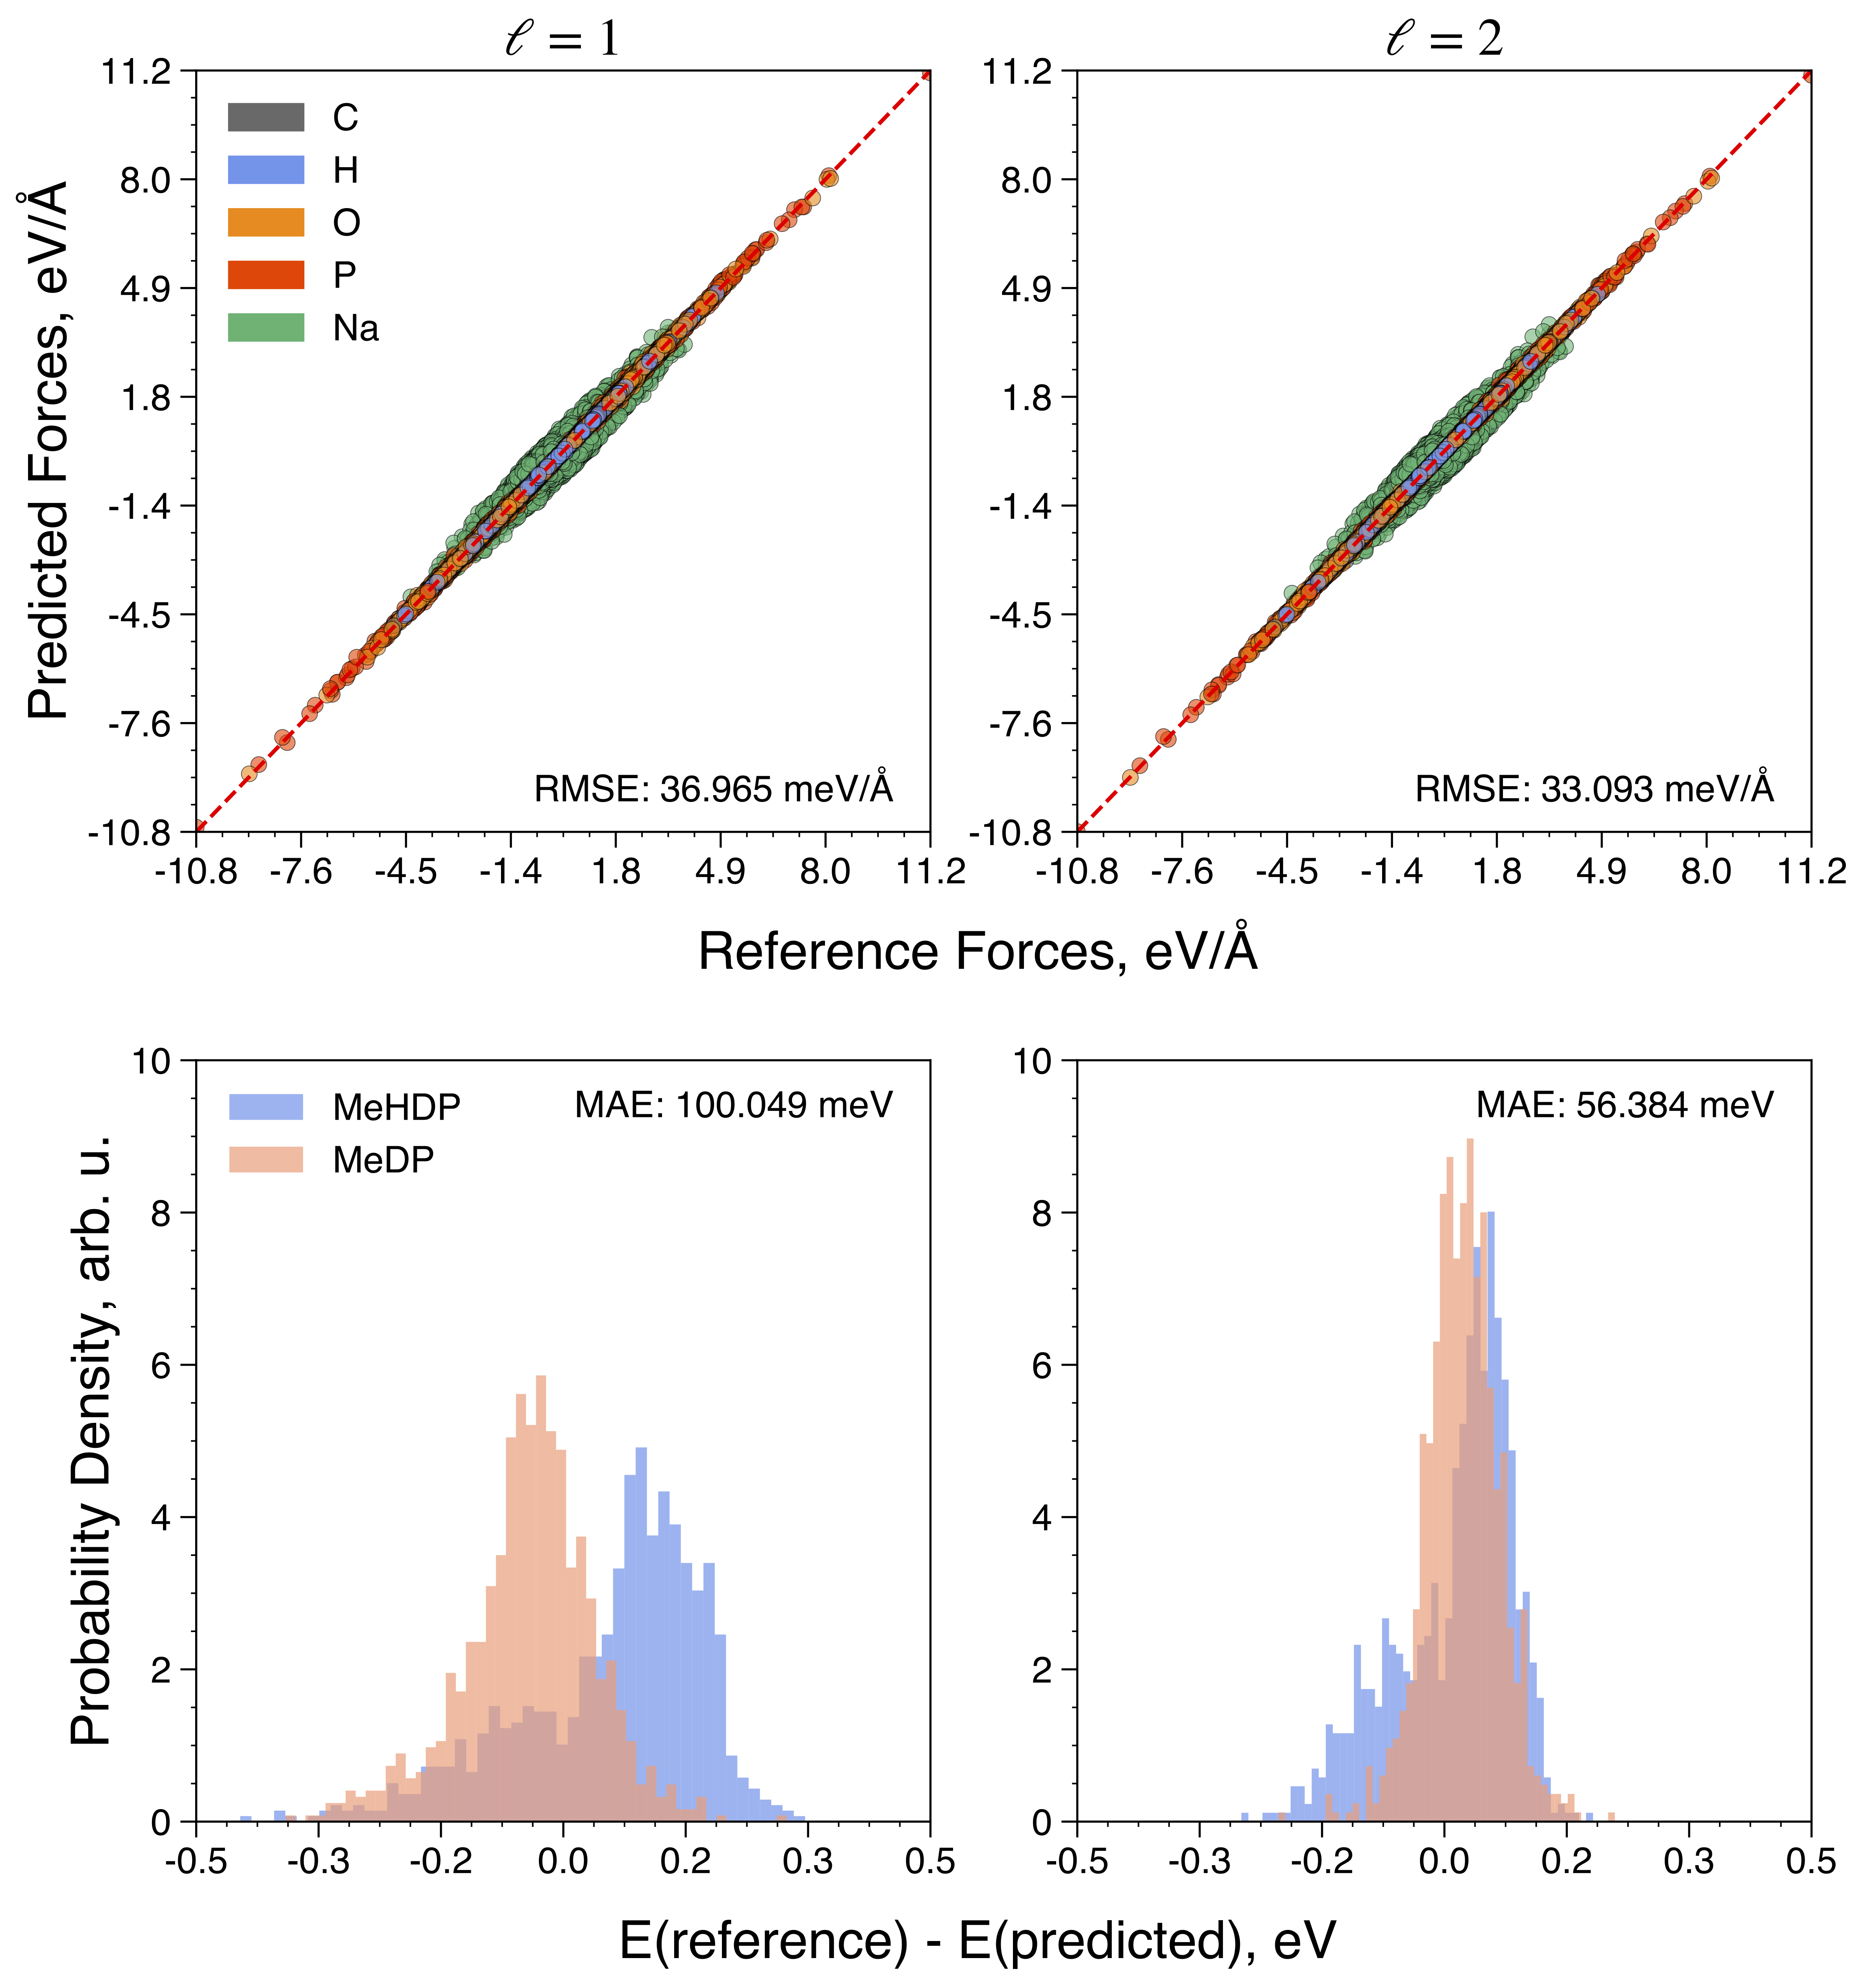
\includegraphics[width=0.8\textwidth]{Figures/4_Results/results_nnp_accuracy_l-1_l-2.png}
    \caption{Accuracy of the neural network potential trained on 12,000 data points. The left panel shows the errors in the forces and energy for the tensor rank $\ell=1$ and the right panel shows the errors for $\ell=2$. The errors are calculated as the difference between the neural network potential and the reference DFT values. For the histograms, the number of bins was set to 50.}
    \label{fig:nnp_accuracy}
\end{figure}

\begin{figure}[htbp]
    \centering
    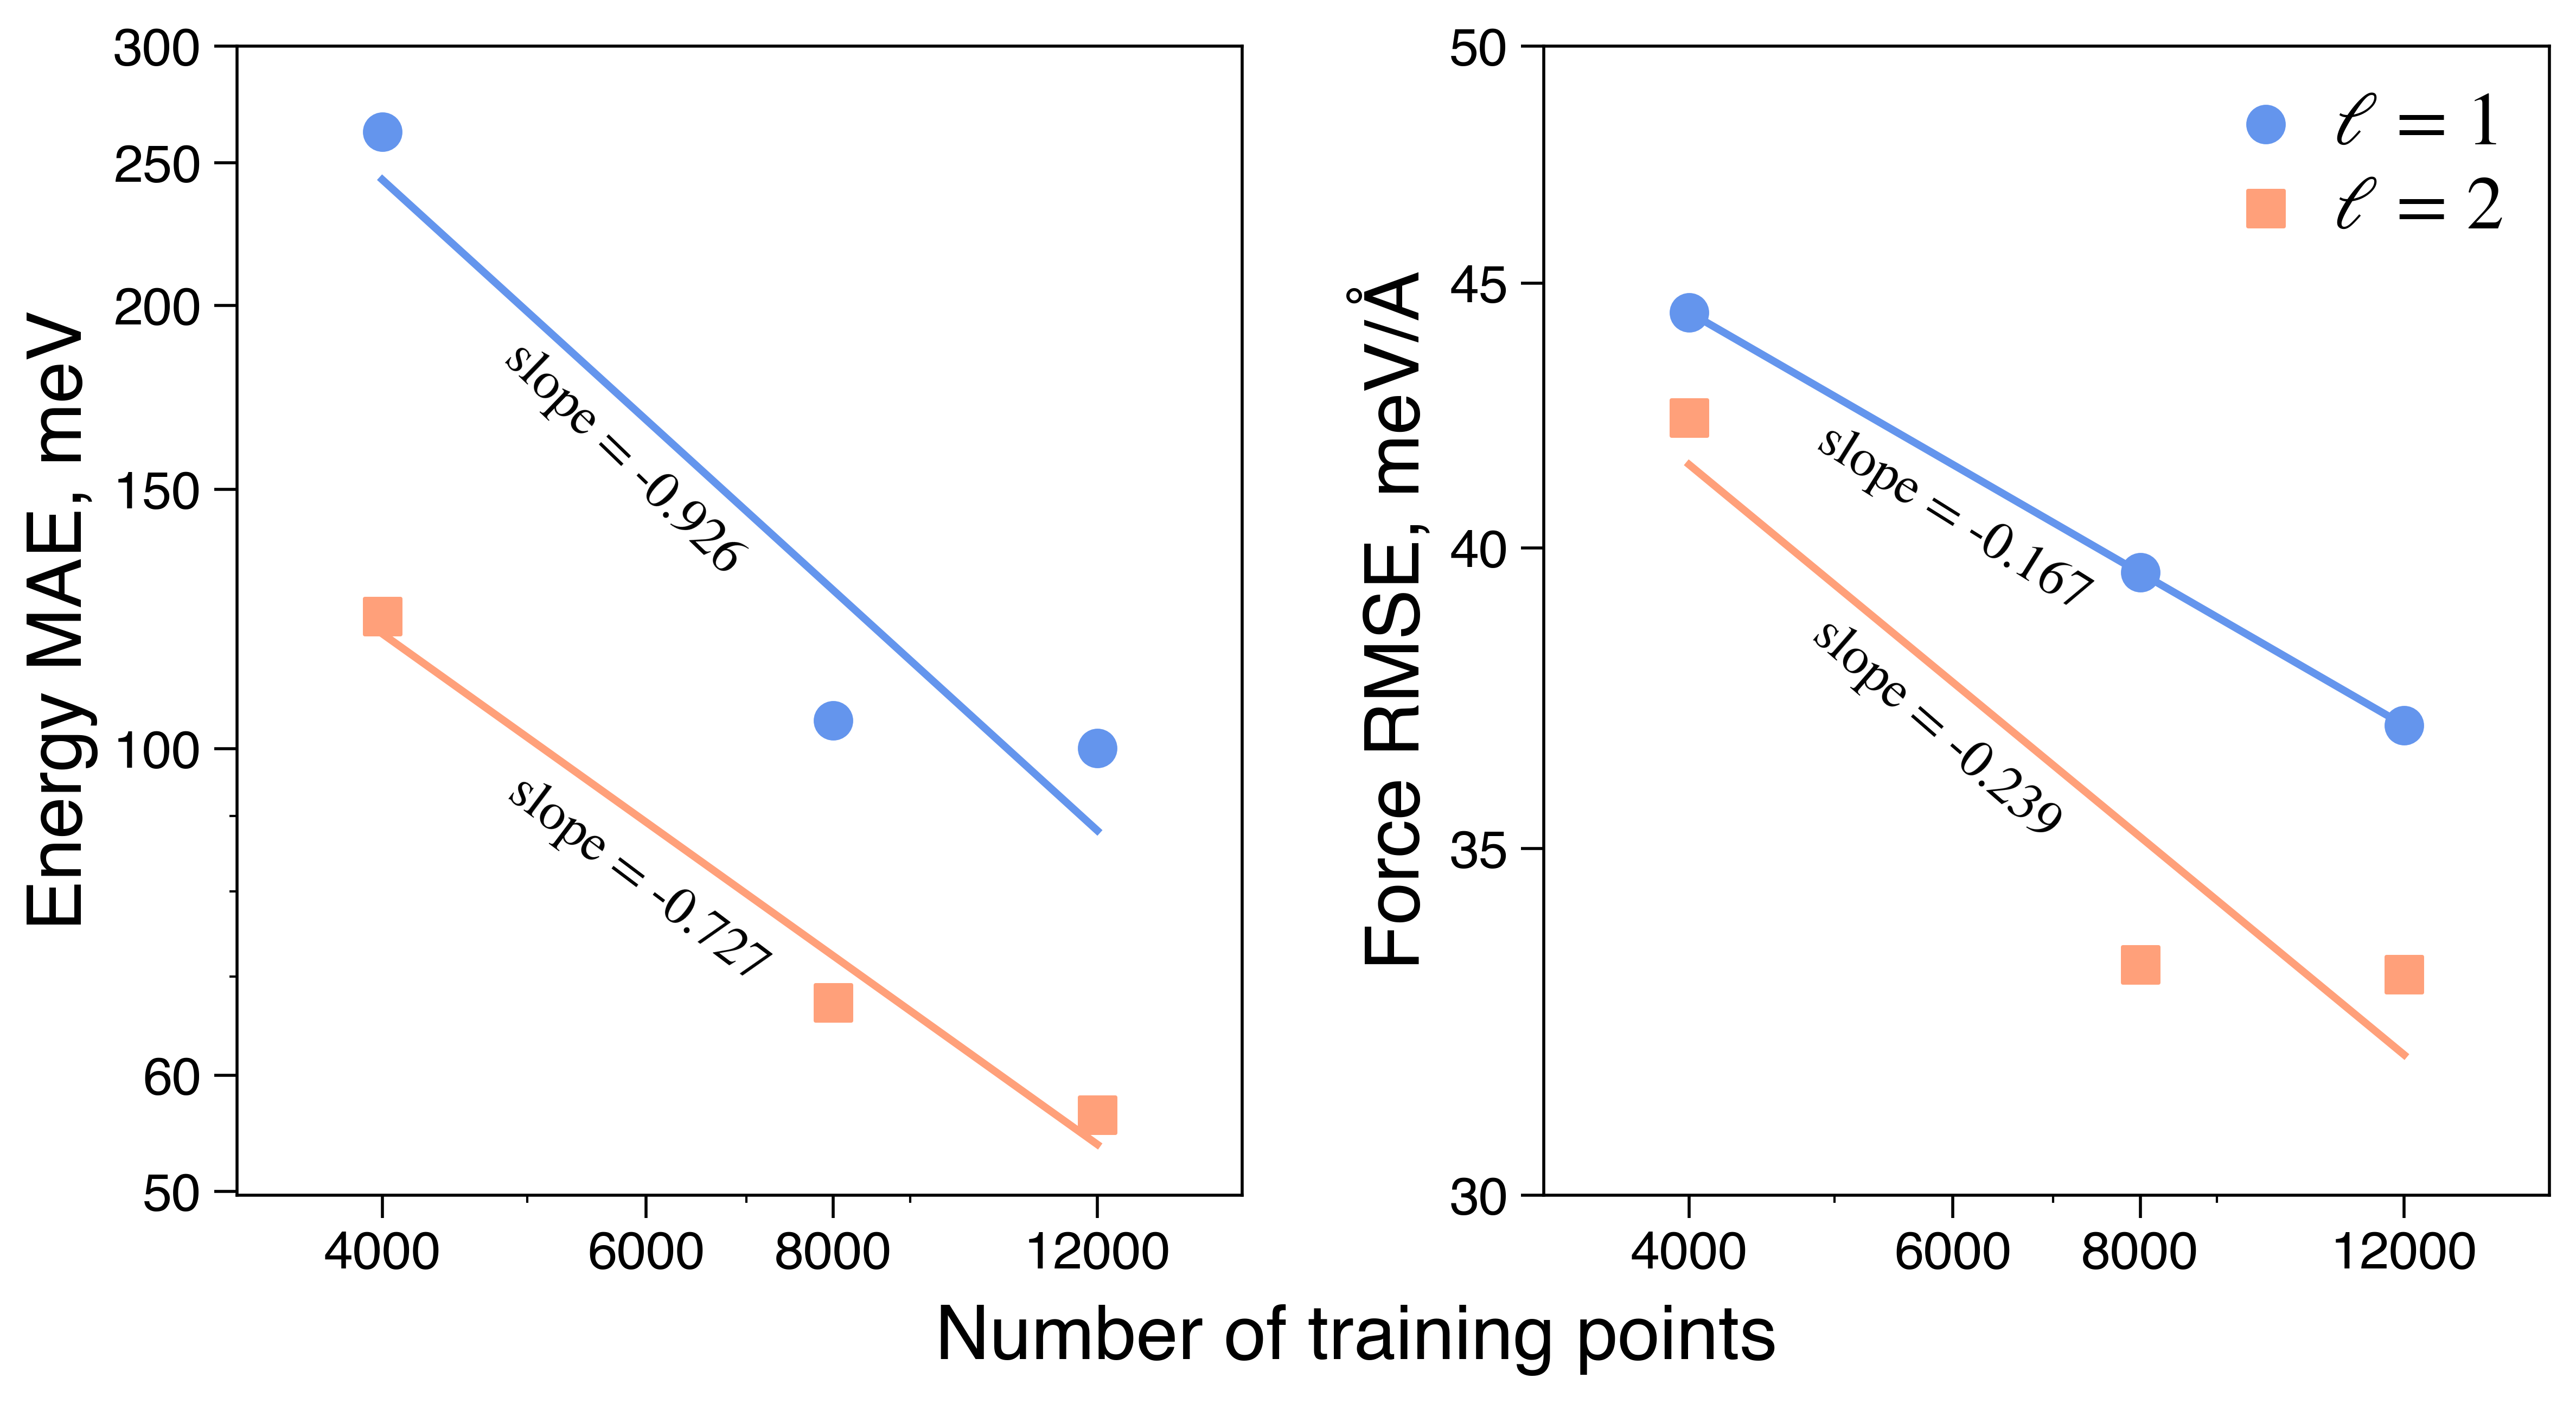
\includegraphics[width=0.8\textwidth]{Figures/4_Results/results_nnp_loglog_energy_force.png}
    \caption{Log-log plot of the errors in the energy and forces for the neural network potential with the respect to the training dataset size. In all cases, the errors were calculated on the final test set of 1,200 data points.}
    \label{fig:nnp_log-log}
\end{figure}
